Lissajous curves were names after Jules Antoine Lissajous. He was French mathematician and physicist who lived from 1822 to 1880. Lissajous studied waves, specifically related to tuning forks. He first explored with tuning forks and water and studying the waves it created. He then moved onto studying acoustic waves using reflected light from a mirror. This study using light in 1855 and figures it created is now known as the Lissajous curves. The apparatus that he build to study the waves, had two tuning forks placed at right angles with mirrors attached to them. The light is then shone on to the first tuning fork, reflecting on the second, and then lastly reflected onto the screen. Depending on the frequency of the tuning forks, the shape created on the screen changes.  Lissajous for his work on "optical observation of vibration", which affects astronomy, physics and other sciences, won the Lacaze Prize in 1873 \cite{JulesAntoineLissajous}.
\begin{figure}[h]
    \centering
    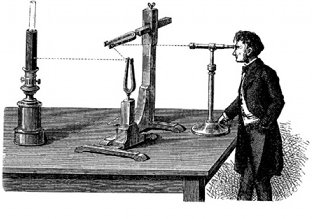
\includegraphics[scale=0.75]{Images/lissajous_obs.jpg}
    \cite{LissajousFigures}
    \caption{"Figure 1: Apparatus built by Lissajous using tuning forks to make Lissajous Curves."}
    \label{fig:my_label}
\end{figure}

Though Lissajous was given credit for these curves, and is most well known for them, Nathaniel Bowditch discovered the curves 1815. Nathaniel Bowditch was born in 1773 in Salem, Massachusetts. Bowditch had to self teach himself calculus, Latin and French due to needing to drop out of school at the age of ten to help his family. He went on to study mathematics, astronomy, and discovered the Bowditch curves - better known as the Lissajous curves now-leading to his fame in the scientific community around the world. Due to his only brief study of the curves, and not as in depth as that of Jules Antoine Lissajous, he is often forgotten as the original discoverer \cite{NathanielBowditch}.
\begin{figure}[h]
    \centering
    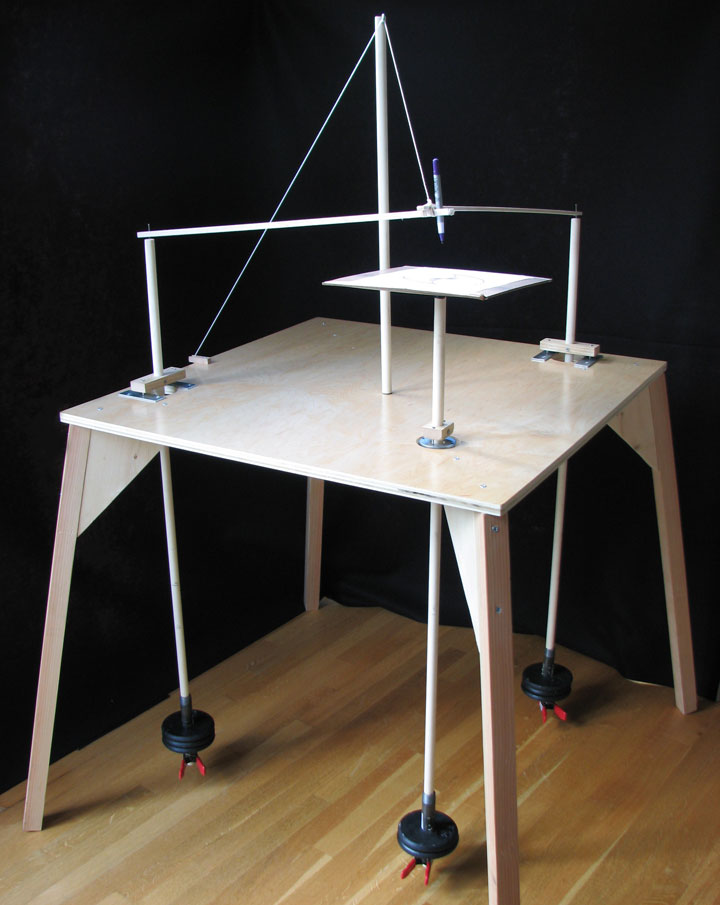
\includegraphics[scale=0.3]{Images/harmonograph.jpg}
    \cite{Harmpic}
    \caption{"Figure 3: Harmonograph."}
    \label{fig:my_label}
\end{figure}

In 1857, Hugh Blackburn, a Scottish mathematician, built the first harmonograph. A harmonograph either has a swinging pencil and or platform, by the means of several pendulums. By pushing the pendulums, one can create "undulating drawings". They are now mostly used for fun, and creating pretty images, as the friction created by the pendulums and the pen dampens the image \cite{Harmonograph}. They can still be analyzed mathematically, but the dampening needs to be accounted for.
\begin{figure}[h]
    \centering
    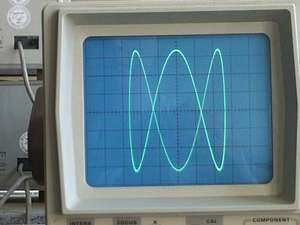
\includegraphics[scale=0.75]{Images/oscilloscope.jpg}\cite{Oscilloscope}
    \caption{"Figure 2: Oscilloscope creating a Lissajous Curve."}
    \label{fig:my_label}
\end{figure}


Lissajous curves can also be created by oscilloscopes, which were invented in 1897. By sending different signals along the X and Y-axis, the image created is that of a Lissajous curve. Using the oscilloscopes one can study the relationship between the frequency, phase, ratio, and amplitude, and the image created\cite{Oscilloscope}.
\newpage
Additionally there is the more modern way of creating and analyzing Lissajous curves through coded programs. Now online it is rather easy to find programs that you plug in all of the variables and it will show you the Lissajous curve that would be created like Figure 4. Furthermore on computers, and with more complex programming, one can create 3D Lissajous curves to analyze shown in Figure 5.

\begin{figure}[h]
    \centering
    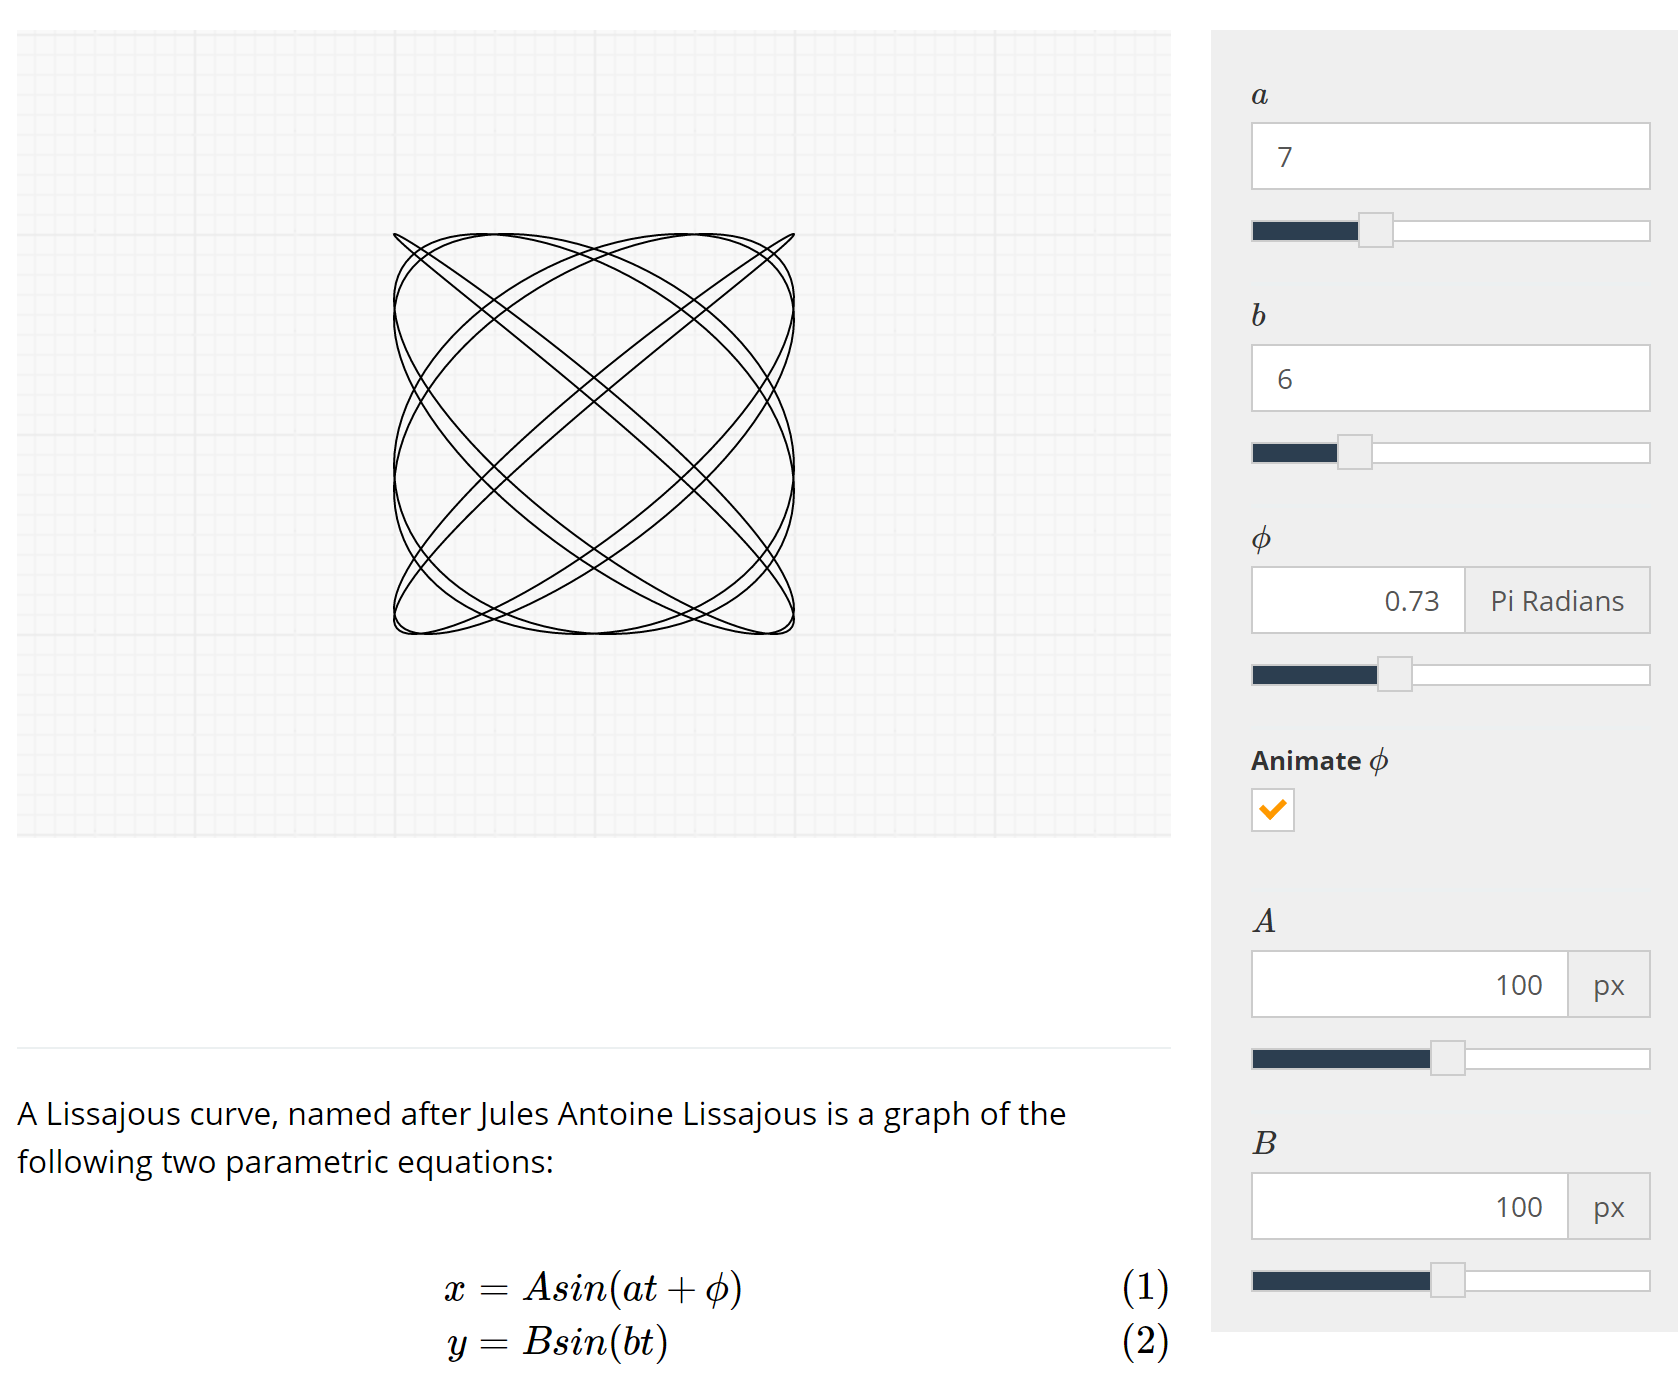
\includegraphics[scale=0.3]{Images/lissajous.PNG}
    \cite{Onlinecurve}
    \caption{"Figure 4: Online program allowing you to plug in all of the variables."}
    \label{fig:my_label}
\end{figure}
\newpage
\begin{figure}[h]
    \centering
    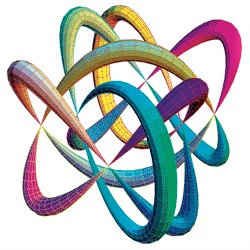
\includegraphics[scale=1.5]{Images/3dcurve.jpg}
    \cite{3DCurve}
    \caption{"Figure 5: 3D Lissajous Curve."}
    \label{fig:my_label}
\end{figure}
